\chapter{Sensor Fusion}
Nei sistemi in cui \`e richiesta un'alta \emph{reliability} delle misure, l'informazione fornita dai singoli sensori non \`e sufficiente. In questi casi \`e raccomandato l'utilizzo di un insieme di sensori in contemporanea.\\*
\section{Panoramica}
In generale, un algoritmo SFA viene utilizzato per stimare lo stato di un sistema dinamico in un ambiente caratterizzato da \emph{rumore}.
\subsection{Sistemi Dinamici}
Un sistema dinamico \`e una modellazione matematica di un processo che evolve nel tempo, la cui evoluzione \`e descritta attraverso un sistema di equazioni differenziali o alle differenze, nel caso esso si evolva rispettivamente a tempo continuo o a tempo discreto.\\*
Sia $S$ l'insieme dei possibili stati che il sistema pu\`o assumere, e sia $m = |S|$ la dimensione dello spazio degli stati.\\*
Senza perdere in generalit\`a, si possono formalizzare questi due tipi di sistemi dinamici come:
$$
y'(t) = f(t,y(t)),\;t\ge 0
$$
Con $y(0) \in \mathbb{R}^m$ condizione iniziale nota, e:
$$
y_{n+1} = f(n,y_n),\;n = 0,1,\dots
$$
con al solito $y_0 \in \mathbb{R}^m$ condizione iniziale nota.\\*
Ricavare lo stato del sistema dinamico per un certo istante $t$, o $n$, equivale a risolvere le equazioni cui sopra e valutarne la traiettoria soluzione in $t$ o in $n$.\\*
Un semplice sistema dinamico \`e rappresentato da un punto materiale che si muove con una accelerazione costante $$\vec{a} = a\vec{k}$$ dove $\vec{k}$ \`e un qualunque versore della base canonica di $\mathbb{R}^3$.\\*
Supponendo che il punto si muova con velocit\`a iniziale $\vec{z'}(0) = v_0\vec{k}$ nota e inizi il moto da una coordinata $\vec z(0) = z_0\vec{k}$ nota, si ha:
$$
z''(t) = a
$$
$$
z'(t) = \int{a dt} = a t + v_0
$$
$$
z(t) = \int(a t + v_0)dt = \frac{1}{2} at^2 +  v_0 t + z_0
$$
L'equazione $z(t)$ descrive completamente la traiettoria di moto del punto materiale, mentre $z'(t)$ descrive completamente la traiettoria della velocit\`a del punto durante il suo moto.
\subsection{Misure e Rumore}
In questo semplice esempio, viene fatta l'assunzione di conoscere a priori il valore esatto di $a$, di $v_0$ e di $z_0$.\\*
Nella pratica, per misurare l'accelerazione $a$ \`e necessario uno strumento denominato \emph{accelerometro}, il quale produrr\`a delle misure giocoforza affette da errori casuali. Si supponga di sostituire $a$ nell'equazione $z(t)$ con una sua perturbazione $\tilde{a} = a + \varepsilon$ dove $\varepsilon$ \`e una variazione casuale della misura data dal \emph{rumore} che caratterizza qualsiasi processo di misura. Si pu\'o supporre $Var(\varepsilon) = 0$ e considerare, ai fini di questa trattazione, $\varepsilon$ come un valore costante; in realt\`a $\varepsilon$ \`e una variable casuale a varianza generalmente non nulla. Si suppongano inoltre $v_0 = z_0 = 0$ per comodit\`a di calcolo:
$$
z(t) = \frac{1}{2} \tilde{a} t^2 = \frac{1}{2}(a + \varepsilon) t^2 = \frac{1}{2} \left(at^2 + \varepsilon t^2\right)
$$
Si nota immediatamente che la variazione della misura $z(t)$ data da $\varepsilon$ aumenta con il quadrato del tempo.\\*
\begin{figure}[h]
	\centering
	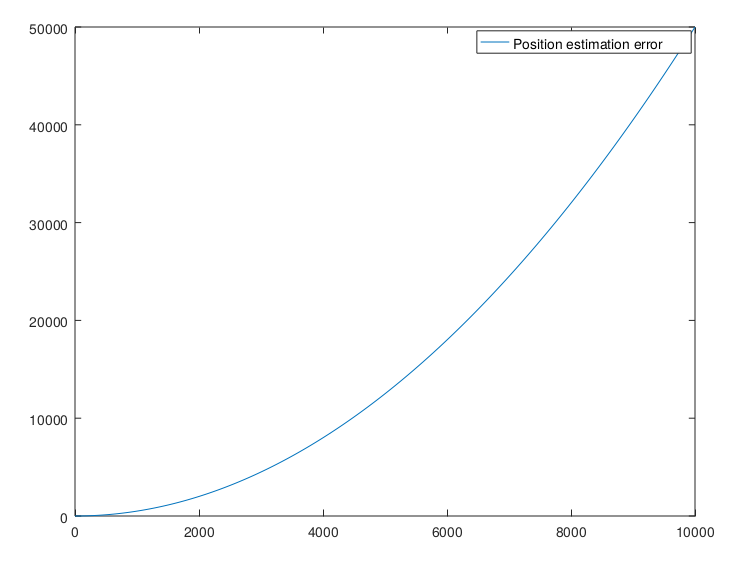
\includegraphics[scale=0.5]{img/errormeas}
	\caption{Grafico dell' errore di stima della posizione con $a = 10^0, \varepsilon = 10^{-3}$}
	\label{fig:errormeas}
\end{figure}
\newpage
\section{I Filtri di Kalman}
Un Filtro di Kalman, o in inglese \emph{Kalman Filter} (KF), \`e un modello di SFA progettato appositamente per risolvere o rendere trascurabile il problema del rumore nei processi di misura.\\*
Siano $X_1,\dots,X_N$ $N$ sorgenti distinte di dati.\\*
Si definisce \emph{misurazione} del valore $j$ dall' $i-$esima sorgente l'osservazione dell'evento:
$$
X_i = j
$$
Per un opportuno $j$ e per $i = 1,\dots,N$.\\*
Modellando ciascuna $X_i$ come una variabile casuale, si ha che ciascuna $X_i$ \`e caratterizzata da una distribuzione di probabilit\`a:
$$
p_{X_i} = \{p_j:P(X_i = j) = p_j\},\;\;\;\;i = 1,\dots,N
$$
Un KF \`e essenzialmente un algoritmo che utilizza una serie di osservazioni $X_i = j$, e cerca di produrre la stima di una \emph{distribuzione di probabilit\`a congiunta} delle variabili casuali $X_i$.
\subsection{Classificazioni}
I KF sono comunemente basati su sistemi dinamici \emph{lineari} a tempo discreto, tuttavia i fenomeni reali sono raramente lineari. Un modello lineare \`e spesso un'approssimazione di un modello pi\`u complesso.\\*
Nel dominio applicativo in cui si colloca la Tesi, ossia quello del posizionamento ferroviario, occorre basare il Filtro di Kalman su un modello non-lineare.
\subsection{Filtri di Kalman Estesi}
\subsubsection{Filtri di Kalman Unscented}